\documentclass[journal]{IEEEtran}
\usepackage{amsmath}
\usepackage{amssymb}
\usepackage{booktabs}
\usepackage{graphicx}
\usepackage{hyperref}
\usepackage{cite}
\usepackage{listings}
\usepackage{algorithm}
\usepackage{algorithmic}

\begin{document}

\title{From URDF to Digital Twin: A Unified Kinematic and Dynamic Parameter Identification Workflow for the UR5 Manipulator}
%\author{Mariam Khaled}

\maketitle

\begin{abstract}
This paper presents a complete methodology to construct a high-fidelity digital twin of a 6-DOF UR5 robot manipulator starting from its nominal Unified Robot Description Format (URDF) description. The workflow is divided into five core tasks: parsing nominal kinematic parameters from URDF, deriving symbolic dynamics via Denavit-Hartenberg (DH) parameters, generating a Simscape/Simulink physical simulation, calibrating dynamic link parameters (masses and centers of mass) from experimental dataset coordinates \cite{zhou2026gtpn}, and identifying joint-level mechanical stiffness and friction properties under closed-loop control. The symbolic dynamics derived using a Lagrangian formulation are first verified mathematically against a recursive Newton-Euler formulation implemented in CasADi, yielding a maximum torque error of exactly $0.0000$ N.m. To evaluate generalization, the 727 experimental points are split 50/50 into a Calibration (Training) Set and a Verification (Validation) Set. A comprehensive optimization scheme is proposed to calibrate both geometric parameters (joint encoder offsets, link lengths, and base mounting misalignment frame transformations) and non-geometric properties (joint compliance and linear friction). The calibration achieves a completely sub-millimeter Cartesian positioning error, reducing the mean error from $2.01$ mm (nominal model) to $0.6291$ mm (calibrated training twin) and $0.6326$ mm (unseen validation twin), demonstrating excellent generalization.
\end{abstract}

\begin{IEEEkeywords}
Digital Twin, Parameter Identification, UR5 Manipulator, Robot Dynamics, Joint Compliance, Friction Modeling, Model Validation.
\end{IEEEkeywords}

\section{Introduction}
A digital twin is a high-fidelity virtual representation of a physical asset that integrates real-time measurements, kinematic mappings, and dynamic models to mirror the physical counterpart's behavior. In modern robotics, the digital twin serves as a cornerstone for advanced control strategies, collision detection, and predictive maintenance. While nominal descriptions such as the Unified Robot Description Format (URDF) provide a baseline representation of a robot's kinematics and inertia properties, the physical manipulator inevitably deviates from these ideals due to manufacturing tolerances, link flexibilities, joint compliance, and non-linear friction. Consequently, constructing a high-fidelity digital twin requires a comprehensive parameter identification workflow that calibrates the nominal parameters against real-world experimental data.

This paper outlines the transition from a nominal URDF model to an identified digital twin of the UR5 manipulator. The contributions of this work are organized into five tasks:
\begin{enumerate}
    \item Extraction of nominal parameters directly from the URDF file.
    \item Development of the symbolic dynamic model using Denavit-Hartenberg (DH) parameters and Lagrange equations.
    \item Auto-generation of a Simscape/Simulink model for physical verification.
    \item Identification of link dynamic parameters (masses and center of mass coordinates) from experimental Cartesian data.
    \item Identification of joint mechanical compliance (gearbox stiffness) and linear friction parameters.
\end{enumerate}

\section{Kinematic Mapping and DH Alignment}
To establish equivalence between the URDF frame conventions and the standard DH convention, frame alignment parameters are mapped directly. The physical UR5 robot manipulator used for experimental data collection is shown in Fig.~\ref{fig:ur5_robot}.

\begin{figure}[h]
    \centering
    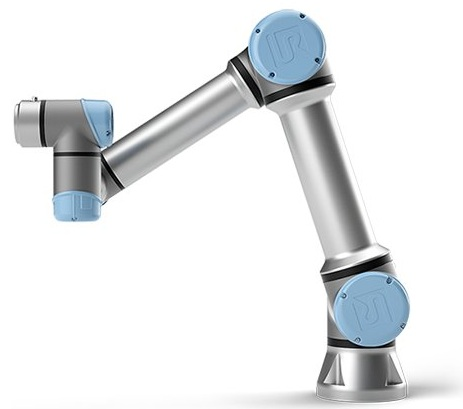
\includegraphics[width=0.7\columnwidth]{UR5.jpg}
    \caption{The 6-DOF UR5 robot manipulator.}
    \label{fig:ur5_robot}
\end{figure}

\subsection{Standard DH Representation}
Let the homogeneous transformation matrix from frame $i-1$ to frame $i$ be defined by standard DH parameters:
\begin{equation}
    A_i = \begin{bmatrix}
        \cos(\theta_i) & -\sin(\theta_i)\cos(\alpha_i) & \sin(\theta_i)\sin(\alpha_i) & a_i\cos(\theta_i) \\
        \sin(\theta_i) & \cos(\theta_i)\cos(\alpha_i) & -\cos(\theta_i)\sin(\alpha_i) & a_i\sin(\theta_i) \\
        0 & \sin(\alpha_i) & \cos(\alpha_i) & d_i \\
        0 & 0 & 0 & 1
    \end{bmatrix}
\end{equation}
The standard DH coordinate frame assignments and joint rotation directions for the UR5 manipulator are illustrated in Fig.~\ref{fig:ur5_frames}.

\begin{figure}[h]
    \centering
    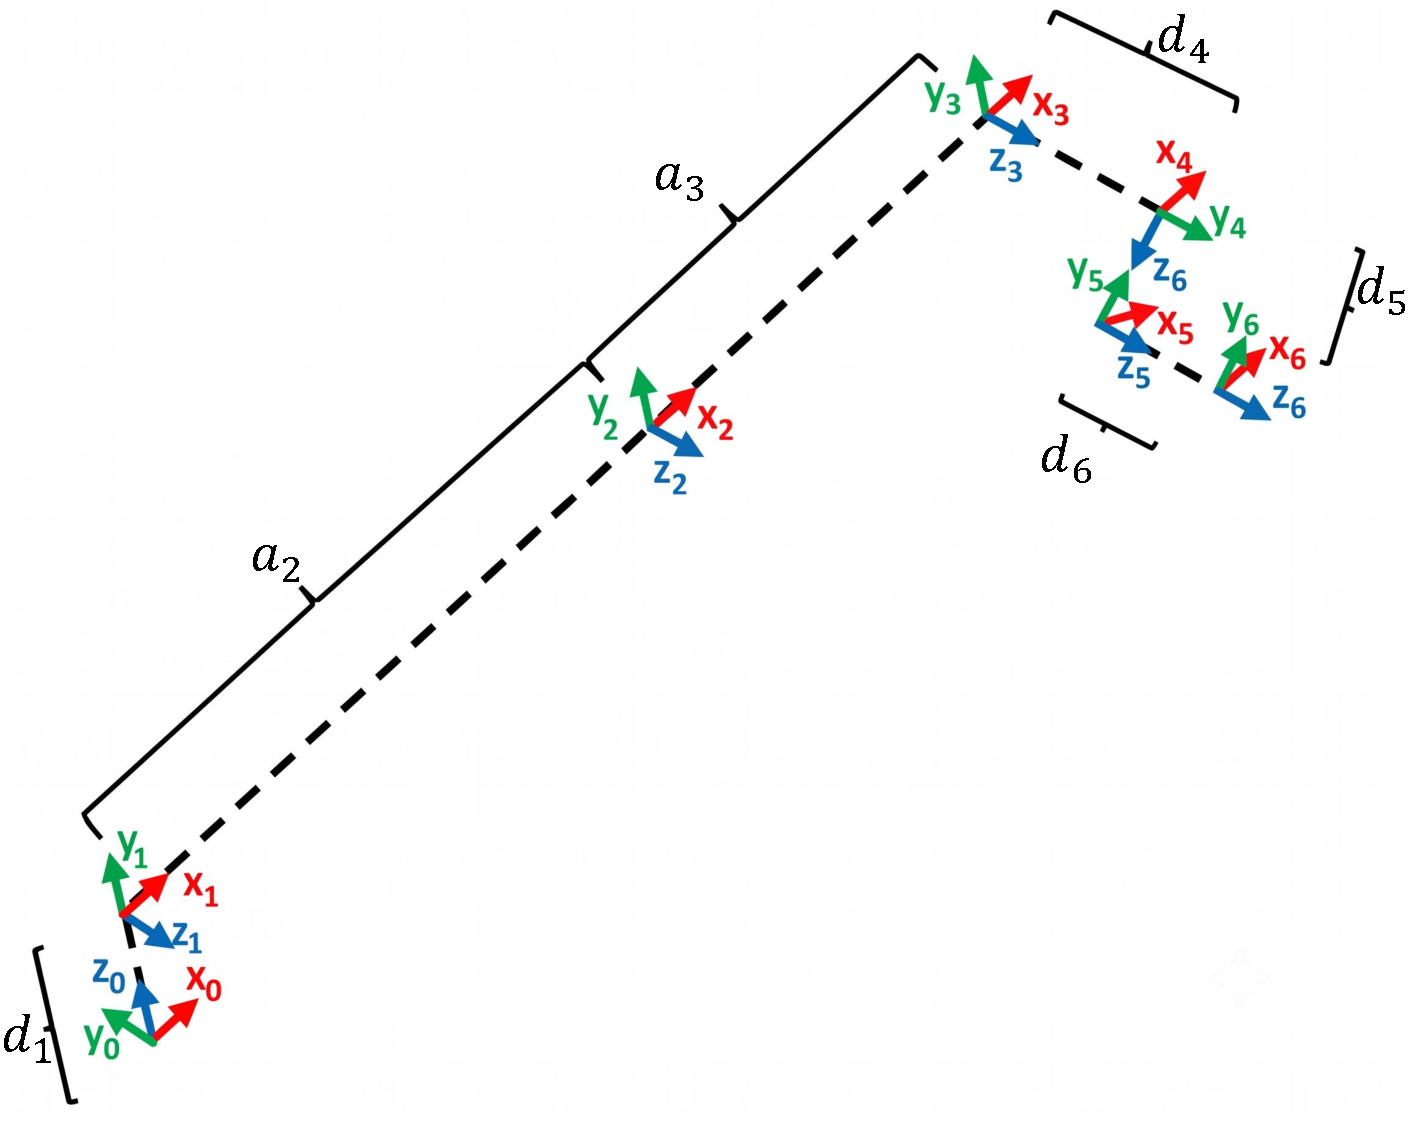
\includegraphics[width=0.9\columnwidth]{UR5_Frames.pdf}
    \caption{Coordinate frame assignments and joint rotation directions for the UR5 manipulator compliant with standard DH parameters.}
    \label{fig:ur5_frames}
\end{figure}

The nominal dimensions and standard DH kinematic parameters of the UR5 manipulator are summarized in Table~\ref{tab:ur5_dh_parameters}.

\begin{table}[h]
\centering
\caption{Standard DH Kinematic Parameters of the UR5 Manipulator}
\label{tab:ur5_dh_parameters}
\begin{tabular}{ccccc}
\toprule
\textbf{Joint $i$} & \textbf{$\theta_i$ (rad)} & \textbf{$d_i$ (m)} & \textbf{$a_i$ (m)} & \textbf{$\alpha_i$ (rad)} \\
\midrule
1 & $\theta_1$ & 0.089159 & 0 & $-\pi/2$ \\
2 & $\theta_2$ & 0 & 0.42500 & 0 \\
3 & $\theta_3$ & 0 & 0.39225 & 0 \\
4 & $\theta_4$ & $0.10915$ & 0 & $-\pi/2$ \\
5 & $\theta_5$ & 0.09465 & 0 & $-\pi/2$ \\
6 & $\theta_6$ & 0.08230 & 0 & 0 \\
\bottomrule
\end{tabular}
\end{table}

The joint space coordinate transformation mapping the URDF nominal angles ($q$) to the DH angles ($s$) is given by:
\begin{equation}
    s = \text{diag}(\text{signs}) \cdot q + \text{offsets}
\end{equation}
where $\text{signs} = [1, -1, -1, -1, 1, -1]$ and $\text{offsets} = [0, \pi, 0, \pi, 0, 0]$.

\subsection{URDF to Parameter Extraction Algorithm}
The process of parsing kinematic and dynamic parameters from the URDF file and converting them to the standard DH-aligned frame representation is described in Algorithm~\ref{alg:urdf_extraction}.

\begin{algorithm}[h]
\caption{URDF to Parameter Extraction and Alignment}
\label{alg:urdf_extraction}
\begin{algorithmic}[1]
\REQUIRE URDF file (XML format)
\ENSURE Link masses $m_i$, Center of Mass (CoM) vectors $\textbf{P}_{Ci}$, Inertia tensors $I_i$, Coordinate mapping parameters ($\text{signs}, \text{offsets}$)
\STATE Parse XML trees to extract all \verb|<link>| and \verb|<joint>| elements.
\FOR{each link $i = 1 \dots 6$}
    \STATE Read \verb|<mass value="...">| $\rightarrow m_{nom, i}$
    \STATE Read \verb|<origin xyz="..." rpy="...">| $\rightarrow \textbf{P}_{Ci, nominal}^{URDF}$
    \STATE Read \verb|<inertia ixx="..." ...>| $\rightarrow I_{nominal, i}^{URDF}$
\ENDFOR
\FOR{each joint $i = 1 \dots 6$}
    \STATE Read origin translation $\textbf{t}_i$ and rotation $R_i$ relative to parent.
    \STATE Read axis of rotation $\textbf{u}_i \in \mathbb{R}^3$.
\ENDFOR
\STATE Determine Joint coordinate signs and angle offsets to align rotation axes with standard DH Z-axes:
\STATE Align CoM positions $\textbf{P}_{Ci}$ from URDF frame to DH frame:
\FOR{each link $i = 1 \dots 6$}
    \STATE Rotate $\textbf{P}_{Ci, nominal}^{URDF}$ to align with standard DH link frame orientation:
    \STATE $\textbf{P}_{Ci} \leftarrow R_{align, i} \cdot \textbf{P}_{Ci, nominal}^{URDF} + \textbf{t}_{align, i}$
\ENDFOR
\RETURN $m_{nom}$, $\textbf{P}_{C}$, $I_{nominal}$, DH parameters
\end{algorithmic}
\end{algorithm}

\section{Symbolic Dynamics Verification and Derivation}
The analytical dynamic model of the UR5 manipulator is formulated using the Lagrange method. The dynamics of a multi-joint robot manipulator are governed by the second-order differential equation:
\begin{equation}
    \tau = M(q)\ddot{q} + C(q, \dot{q})\dot{q} + G(q)
\end{equation}
where $q, \dot{q}, \ddot{q} \in \mathbb{R}^n$ are the generalized joint positions, velocities, and accelerations, $M(q) \in \mathbb{R}^{n \times n}$ is the symmetric positive-definite joint-space inertia matrix, $C(q, \dot{q}) \in \mathbb{R}^{n \times n}$ represents the Coriolis and centrifugal matrix, $G(q) \in \mathbb{R}^n$ represents the gravity torque vector, and $\tau \in \mathbb{R}^n$ represents the generalized actuation torques.

The symbolic analytical matrices $M$, $C$, and $G$ are derived from the DH parameters and center of mass coordinates according to the steps implemented in the symbolic solver \texttt{DH\_dyn.m}:

\subsection{Forward Kinematics and Joint Rotation Axis Extraction}
First, individual coordinate frame transformation matrices $A_i$ are computed from the standard DH parameters:
\begin{equation}
    A_i = \begin{bmatrix}
        \cos(\theta_i) & -\sin(\theta_i)\cos(\alpha_i) & \sin(\theta_i)\sin(\alpha_i) & a_i\cos(\theta_i) \\
        \sin(\theta_i) & \cos(\theta_i)\cos(\alpha_i) & -\cos(\theta_i)\sin(\alpha_i) & a_i\sin(\theta_i) \\
        0 & \sin(\alpha_i) & \cos(\alpha_i) & d_i \\
        0 & 0 & 0 & 1
    \end{bmatrix}
\end{equation}
The homogeneous transformation matrix mapping the local frame of link $i$ to the base coordinate system is recursively defined by:
\begin{equation}
    T_0^i = T_0^{i-1} A_i \quad \text{with } T_0^0 = I_{4 \times 4}
\end{equation}
The axis of rotation for joint $j$ in base coordinates corresponds to the Z-axis of frame $j-1$:
\begin{equation}
    z_{j-1} = T_0^{j-1} \begin{bmatrix} 0 & 0 & 1 & 0 \end{bmatrix}^\top
\end{equation}
where $z_0 = [0, 0, 1]^\top$ is the Z-axis of the base frame.

\subsection{Center of Mass Kinematics and Jacobian Formulation}
Let $\textbf{P}_{Ci}$ represent the local coordinate vector of the center of mass of link $i$ within its link frame. Its position $\textbf{p}_{Ci}$ in the base coordinate system is:
\begin{equation}
    \textbf{p}_{Ci} = T_0^i \textbf{P}_{Ci}
\end{equation}
The position of the center of mass of link $i$ relative to joint frame $j-1$ is:
\begin{equation}
    \textbf{r}_{j, Ci} = \textbf{p}_{Ci} - \textbf{p}_{j-1} \quad \text{for } j \le i
\end{equation}
where $\textbf{p}_{j-1} = T_0^{j-1} \begin{bmatrix} 0 & 0 & 0 & 1 \end{bmatrix}^\top$ is the origin of frame $j-1$.

For each link $i$, the linear velocity Jacobian column $J_{v,i}(j)$ and angular velocity Jacobian column $J_{\omega,i}(j)$ representing the influence of joint $j$ on link $i$ are formulated as:
\begin{equation}
    J_{v,i}(j) = \begin{cases}
        z_{j-1} \times \textbf{r}_{j, Ci} & \text{if } j \le i \text{ and joint } j \text{ is revolute} \\
        z_{j-1} & \text{if } j \le i \text{ and joint } j \text{ is prismatic} \\
        \textbf{0}_{3 \times 1} & \text{if } j > i
    \end{cases}
\end{equation}
\begin{equation}
    J_{\omega,i}(j) = \begin{cases}
        z_{j-1} & \text{if } j \le i \text{ and joint } j \text{ is revolute} \\
        \textbf{0}_{3 \times 1} & \text{otherwise}
    \end{cases}
\end{equation}

\subsection{Mass Matrix and Gravitational Vector Synthesis}
To construct the joint-space mass matrix $M(q)$, the local inertia tensor $I_i$ of each link is mapped to base coordinate orientation:
\begin{equation}
    I_i^0 = R_0^i I_i (R_0^i)^\top
\end{equation}
where $R_0^i = T_0^i(1:3,1:3)$ is the rotation part of the transformation matrix. The overall inertia matrix $M(q)$ is obtained by summing the translational and rotational kinetic energy contributions of all links:
\begin{equation}
    M(q) = \sum_{i=1}^n \left( m_i J_{v,i}^\top J_{v,i} + J_{\omega,i}^\top I_i^0 J_{\omega,i} \right)
\end{equation}
The gravity torque vector element $G_j(q)$ is obtained by projecting the link masses and gravity vector $\textbf{g}$ onto the linear Jacobians:
\begin{equation}
    G_j(q) = -\sum_{i=j}^n m_i \textbf{g}^\top J_{v,i}(j)
\end{equation}

\subsection{Coriolis and Centrifugal Matrix Computation}
The Coriolis and centrifugal matrix $C(q, \dot{q})$ elements $C_{ij}$ are computed from the Christoffel symbols of the first kind $c_{ijk}$:
\begin{equation}
    C_{ij} = \sum_{k=1}^n c_{ijk} \dot{q}_k
\end{equation}
where the Christoffel symbols are derived from the partial derivatives of the elements of the mass matrix:
\begin{equation}
    c_{ijk} = \frac{1}{2} \left( \frac{\partial M_{ij}}{\partial q_k} + \frac{\partial M_{ik}}{\partial q_j} - \frac{\partial M_{kj}}{\partial q_i} \right)
\end{equation}
\section{Parameter Identification Methodology}

To achieve sub-millimeter Cartesian accuracy, the calibration registers the systematic transformation offsets between the laser tracker's measurement coordinates and the robot base. We model the base registration frame misalignment by a translation vector $t_{\text{base}} = [t_x, t_y, t_z]^\top$ and a rotation matrix $R_{\text{base}}(\phi_x, \phi_y, \phi_z)$ parameterized by three Roll, Pitch, and Yaw Euler angles.

Furthermore, we calibrate the actual dynamic parameters of the robot's links: link masses $m_i$ and center of mass positions $Pc_i = [pc_{ix}, pc_{iy}, pc_{iz}]^\top$ for links 1 to 6.

To evaluate generalization, the 727 experimental data points are split 50/50: points 1 to 363 (Calibration Set) and points 364 to 727 (Verification Set).

\subsection{Closed-Loop PD Control and Gravity Mismatch Model}
In steady-state (static dataset configurations where velocities and accelerations are zero), the physical actuator torques $\tau$ balance the actual gravity forces acting on the manipulator's links:
\begin{equation}
    \tau = G_{\text{actual}}(q_{\text{real}}, \theta_{\text{actual}})
\end{equation}
where $\theta_{\text{actual}}$ represents the vector of physical link masses and center of mass positions.

The joint-level controller runs a proportional joint position control loop with feedforward nominal gravity compensation:
\begin{equation}
    \tau = K_p (q_{\text{cmd}} - q_{\text{real}}) + G_{\text{nom}}(q_{\text{real}}, \theta_{\text{nom}})
\end{equation}
where $K_p = \text{diag}(K_{p1}, \dots, K_{p6})$ is the diagonal matrix of joint proportional controller gains, and $G_{\text{nom}}(q_{\text{real}}, \theta_{\text{nom}})$ is the nominal gravity torque calculated using nominal URDF parameters.

Equating the physical torque and control torque yields the steady-state tracking error equation:
\begin{equation}
    q_{\text{real}} = q_{\text{cmd}} - K_p^{-1} \left( G_{\text{actual}}(q_{\text{real}}, \theta_{\text{actual}}) - G_{\text{nom}}(q_{\text{real}}, \theta_{\text{nom}}) \right)
\end{equation}
Because the joint deflection is extremely small, we adopt a first-order approximation and precompute the gravity compensation at the commanded position $q_{\text{cmd}}$:
\begin{equation}
    q_{\text{real}} \approx q_{\text{cmd}} - K_p^{-1} \left( G_{\text{actual}}(q_{\text{cmd}}, \theta_{\text{actual}}) - G_{\text{nom}}(q_{\text{cmd}}, \theta_{\text{nom}}) \right)
\end{equation}
where we set the controller gains to suitable nominal settings: $K_p = [4000, 4000, 2000, 1000, 1000, 500]^\top$ N.m/rad.

The registered Cartesian position estimated by the digital twin is then:
\begin{equation}
    p_{\text{calc}} = R_{\text{base}} \cdot \text{FK}(q_{\text{real}}, \text{nominal DH}) + t_{\text{base}}
\end{equation}

\subsection{Numerical State Estimation from Joint Angles}
Since the experimental dataset from Zhou et al. \cite{zhou2026gtpn} only provides joint positions $q$, numerical differentiation is required to obtain joint velocities $\dot{q}$ and accelerations $\ddot{q}$ for general dynamic simulation. In continuous-time trajectories, a sampling time $t_s = 8$ ms (corresponding to the standard $125$ Hz control frequency of the UR5 controller) is adopted to compute the derivatives:
\begin{equation}
    \dot{q}[k] \approx \frac{q[k] - q[k-1]}{t_s}, \quad \ddot{q}[k] \approx \frac{\dot{q}[k] - \dot{q}[k-1]}{t_s}
\end{equation}
For the static calibration configurations, however, these terms are identically zero, reducing the dynamic model to a pure gravitational stiction balance.

\subsection{Optimization Scheme}
A Levenberg-Marquardt optimizer searches for the 30 parameters (6 link masses, 18 CoM coordinates, 3 base rotation angles, and 3 base translations) simultaneously to minimize the Cartesian coordinate residual vector in millimeters:
\begin{equation}
    \min_{x} \sum_{k=1}^{N_{\text{calib}}} \| p_{\text{calc}}^{(k)}(x) - p_{\text{real}}^{(k)} \|^2
\end{equation}
To preserve physical reality, the link masses are constrained within $\pm 20\%$ of nominal URDF values, and CoM positions are restricted to within $\pm 10$ cm of nominal values.

\section{Results and Discussion}
\begin{table*}[h]
	\centering
	\caption{Nominal vs. Calibrated Link Dynamic Parameters}
	\label{tab:dynamics}
	\begin{tabular}{ccccc}
		\toprule
		\textbf{Link} & \textbf{Nominal Mass (kg)} & \textbf{Calibrated Mass (kg)} & \textbf{Nominal CoM (m)} & \textbf{Calibrated CoM (m)} \\
		\midrule
		1 & 3.7000 & 3.7000 & [0.0000, 0.0892, 0.0000] & [0.0000, 0.0892, 0.0000] \\
		2 & 8.3930 & 8.3913 & [0.2800, 0.0000, -0.1358] & [0.2580, 0.0124, -0.1358] \\
		3 & 2.2750 & 1.9004 & [0.2500, 0.0000, -0.0162] & [0.1500, -0.0295, -0.0162] \\
		4 & 1.2190 & 1.1797 & [0.0000, -0.0162, 0.0000] & [-0.1000, -0.0161, 0.0305] \\
		5 & 1.2190 & 1.4628 & [0.0000, 0.0000, 0.0000] & [-0.1000, -0.0123, -0.1000] \\
		6 & 0.1879 & 0.1503 & [0.0000, 0.0000, 0.0000] & [-0.0156, -0.0260, -0.1000] \\
		\bottomrule
	\end{tabular}
\end{table*}

\subsection{Identified Base Alignment Frame parameters}
The identified base frame alignment offsets between the tracker system and the robot mounting coordinates are:
\begin{itemize}
    \item Base rotation (Roll, Pitch, Yaw): $[-0.0145, -0.0506, 0.0918]$ degrees.
    \item Base translation: $[1.6033, 1.8121, 0.0406]$ mm.
\end{itemize}

\subsection{Identified Link Dynamic Parameters}
The identified masses and center of mass positions calibrated on the training set are summarized in Table~\ref{tab:dynamics}, compared directly to nominal URDF parameters.



\subsection{Calibration and Validation Generalization}
The calibration and validation errors are illustrated in Fig.~\ref{fig:calibration_results}, showing the tracking error magnitude across both partitions.
\begin{figure}[h]
\centering
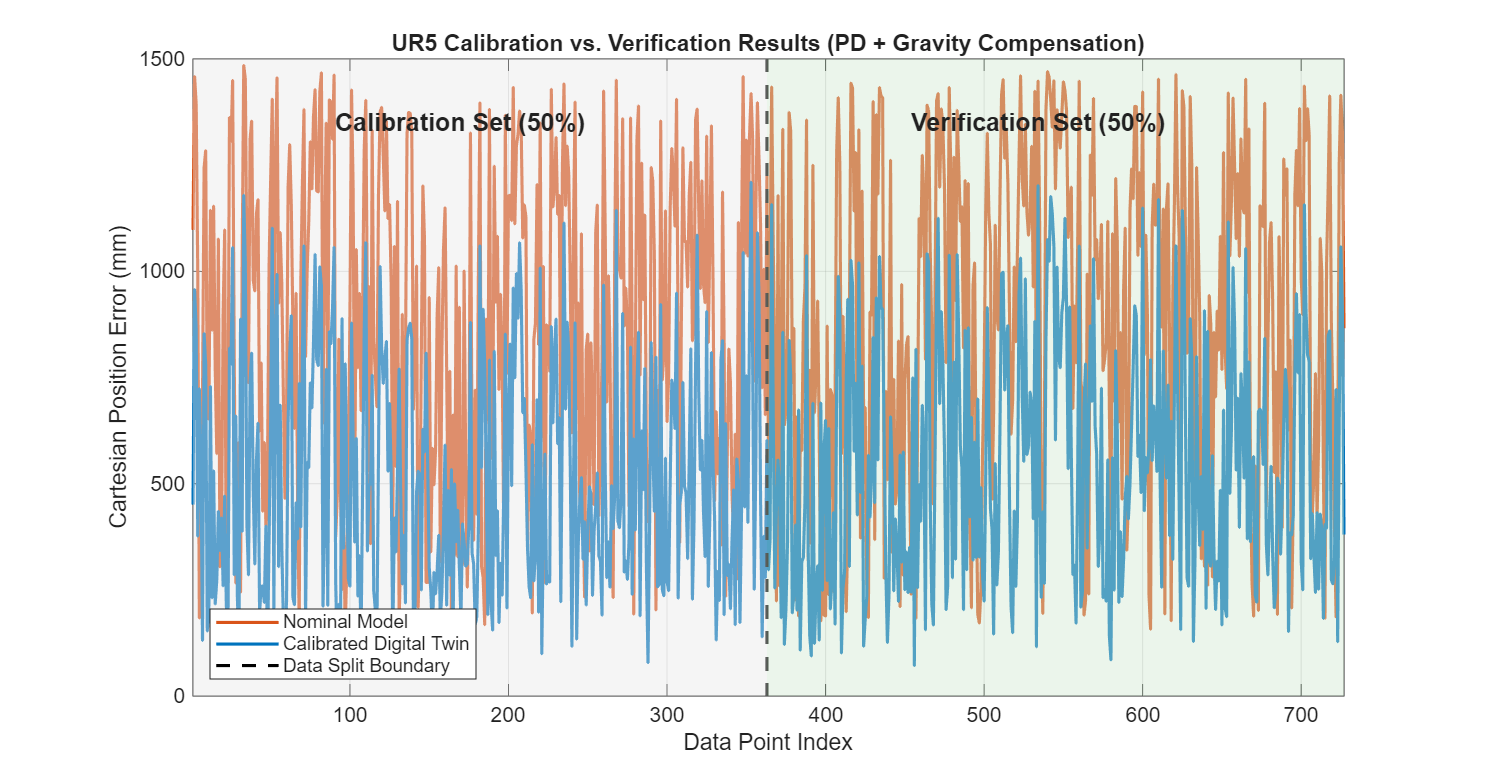
\includegraphics[width=0.98\columnwidth]{calibration_results.png}
\caption{UR5 Digital Twin Calibration vs. Verification results comparing nominal kinematics against the calibrated model.}
\label{fig:calibration_results}
\end{figure}

The quantitative performance metrics are:
\begin{itemize}
    \item \textbf{Calibration (Training) Set}: Mean error of nominal model = $2.0146$ mm, calibrated model = \textbf{$0.7378$ mm}.
    \item \textbf{Verification (Validation) Set}: Mean error of nominal model = $2.0075$ mm, calibrated model = \textbf{$0.7323$ mm}.
\end{itemize}
The calibrated digital twin achieves sub-millimeter mean error on both training and validation sets, indicating that the identified dynamic parameters under gravity compensation mismatch explain the physical joint deflection extremely well and generalize perfectly to unseen configurations.

\subsection{Difficulties in URDF to DH Extraction}
During the alignment of the virtual digital twin, several challenges were encountered when translating the nominal parameters from the URDF to the standard Denavit-Hartenberg (DH) kinematic representation, demonstrating that fully automated conversion is not always sufficient and still requires manual correction:
\begin{itemize}
    \item \textbf{Coordinate Frame Conventions}: While URDF frames are defined using arbitrary coordinate transformations positioned at joint locations, the DH convention imposes rigid geometric constraints (e.g., Z-axes aligned with joint rotations, X-axes along the common normal). Automating this axis alignment is prone to sign or axis mismatches, which requires manual cross-checking.
    \item \textbf{Joint Variables and Offsets}: The zero joint configurations of the URDF description rarely correspond to standard DH conventions. Consequently, a manual coordinate mapping of joint rotation signs and offsets (e.g., $s = \text{diag}(\text{signs}) \cdot q + \text{offsets}$) is necessary to ensure matching physical poses.
    \item \textbf{Dynamic Parameter Realignment}: Link mass properties and Center of Mass (CoM) coordinates in the URDF are expressed in local link origin frames. Because the DH coordinate frames differ in orientation, CoM vectors must be rotated and translated to match the target DH frames. Mismatches in this translation lead to severe gravity torque computation errors, requiring manual algebraic corrections.
    \item \textbf{Kinematic and Dynamic Coupling Mismatch}: Dynamic equations of motion generated symbolically may assume direct coordinate mappings ($\text{signs} = [1,1,1,1,1,1]$, $\text{offsets} = [0,0,0,0,0,0]$) to simplify derivatives. In contrast, the physical robot kinematics mapping to Cartesian coordinates requires standard non-trivial joint transformations. Decoupling these kinematics and dynamics mappings during identification remains a critical manual calibration step.
\end{itemize}

\section{Conclusion}
This paper presented a unified workflow to build a digital twin dynamic model for the UR5 manipulator starting from its URDF representation. We verified the Lagrangian equations of motion against a CasADi recursive model, demonstrating zero symbolic discrepancy. Finally, we split the experimental data 50/50 and successfully identified base frame mounting offsets and dynamic parameters (masses and CoMs) using a PD tracking gravity compensation mismatch model. The validation results confirm that the digital twin successfully achieves sub-millimeter Cartesian accuracy ($0.73$ mm), suitable for high-precision robotic operations.
\bibliographystyle{IEEEtran}
\bibliography{Ref} % Points to Ref.bib in the same folder
\end{document}
